\chapter{Testes} \label{cap:cap5}

Foram feitos testes em três fases distintas do desenvolvimento do ambiente de simulação aqui desenvolvido. 
Todas como parte do projeto aprovado no comitê de ética do Hospital Universitário Antônio Pedro associado a faculdade de medicina da Universidade Federal Fluminense. Este projeto foi registrado na Plataforma Brasil do ministério da saúde sob o número 23637019.5.0000.5243 (texto no apêndice \ref{apend:comiteEtica}). A primeira fase de testes envolveu avaliações das sensações proporcionadas pelo dispositivo háptico. A segunda e a terceira fase foram feitas em paralelo com todo o ambiente de simulação já desenvolvido. A segunda fase foi um teste de usabilidade e a terceira uma avaliação do ambiente como um todo por especialistas.
A Tabela~\ref{tab:tabelaCaracteristicasVoluntarios} detalha as características dos voluntários que participaram dos testes em cada fase.

\begin{table}[!ht]
\begin{center}
\caption{Características dos voluntários dos testes em cada fase.}
\label{tab:tabelaCaracteristicasVoluntarios}
\begin{tabular}{|p{0.4\linewidth}|p{0.15\linewidth}|p{0.15\linewidth}|p{0.15\linewidth}|}
\hline
\textbf{n=84} & \textbf{Fase 1 - Estudantes de computação} & \textbf{Fase 2 - Estudantes de computação} & \textbf{Fase 3 - Médicos anestesistas}\\
\hline\hline
Tamanho da população, n & 12 & 62 & 10\\
Homens, n (\%) & 11 (92\%) & 50 (81\%) &  5 (50\%)\\
Experiência anterior com RV, n(\%) & 7 (58\%)  & 37 (60\%) & 3 (30\%) \\
\hline
\end{tabular}
\end{center}
\end{table}

\section{Simulação das sensações}
\label{sec:testeSensacoes}

Esta seção detalha os experimentos para avaliação do correto reconhecimento das sensações hápticas necessárias de serem simuladas para a reprodução do procedimento de raquianestesia. Os resultados destes experimentos são descritos ao final. A descrição destes experimentos e discussão dos resultados obtidos foram publicados em conferência da área \cite{Melo2021}. 

Os experimentos foram apresentados a doze voluntários que fizeram uso do equipamento háptico, todos estes voluntários eram estudantes de ciência da computação com idades variando entre 18 e 44 anos sendo onze homens e uma mulher. Todos os voluntários concordaram com o termo de consentimento de participação nesta pesquisa e receberam uma breve explicação (cinco minutos) a respeito do procedimento de uso do equipamento háptico no experimento. Em seguida tiveram outros cinco minutos de tempo para usar um aplicativo de exemplo (para adquirir conhecimento sobre como interagir num ambiente com este tipo de dispositivo) visando nivelar o conhecimento. Para construir critérios mais objetivos, nesta tese focamos nossos experimentos em fazer perguntas com respostas esperadas em vez de questionários para validar as opiniões dos usuários. As respostas indicam se um comportamento específico pode ser mapeado corretamente.

Conforme comentado na seção anterior utilizamos o \textit{Haptic Plug-In For Unity3D} para programação das interações com o háptico utilizando o motor de jogo da \textit{Unity} \cite{UnityTechnologies2020} que é uma ferramenta muito utilizada para desenvolvimento de videogames e simulações com e sem \acrshort{RV} para diversas plataformas.
Este \textit{plugin} possibilita a interação do usuário com os objetos no ambiente virtual  de quatro modos distintos \cite{Poyade2014}. Para este experimento utilizamos o modo \textit{Puncture} (modo de punção) pelo requisito do experimento em simular uma agulha sendo inserida através de camadas representativas de tecidos.

O \textit{OpenHaptics driver} possui a definição de um conjunto de propriedades que representam como qualquer objeto 3D (camada, superfície, etc) tocável do ambiente virtual desenvolvido reage a cada interação com o dispositivo háptico. As propriedade mais relevantes no contexto do modo de punção são \textit{Stiffness}, \textit{Pop Through}, \textit{Static Friction}, e \textit{Dynamic Friction}. Todas elas têm como domínio um número real e aceitam valores entre zero e um. 

\textit{Stiffness} representa o nível de dureza do objeto: zero (0) representa um objeto mole e um (1) o objeto mais duro possível \cite{3DSystemsTouch2018}. Neste ponto é importante ressaltar que a quantidade de força máxima suportada depende das especificações do dispositivo háptico usado, dispositivos mais simples e de custo mais baixo comumente suportam intensidades de forças menores se comparadas a dispositivos mais complexos e com custos mais altos. \textit{Pop Through} controla o nível de força necessária para perfurar um objeto: zero indica que o objeto não pode ser perfurado e um que o máximo de força é necessário para perfurar o objeto \cite{3DSystemsTouch2018}. \textit{Punctured Static Friction} configura a dificuldade de se mover dentro de um objeto perfurado a partir de uma posição estática. O limite inferior (zero) representa um movimento sem atrito e o limite superior (um) representa a quantidade maior de atrito suportada pelo dispositivo \cite{3DSystemsTouch2018}. \textit{Punctured Dynamic Friction} controla a dificuldade de se mover dentro de um objeto depois que o movimento já foi iniciado \cite{3DSystemsTouch2018}. Da mesma forma que no caso estático o zero representa um movimento sem atrito e um o máximo de atrito suportado. Essas propriedades podem ser usadas para configurar o comportamento de cada camada de forma que o usuário tenha um experiência tátil de interação virtual que simule o procedimento real. As propriedades \textit{Stiffness} e \textit{Pop Through} precisam ser configuradas pra se determinar a força necessária por parte do usuário para perfurar cada objeto enquanto para determinar a força necessária para movimentação de uma agulha dentro de um objeto as propriedade a serem configuradas são \textit{Punctured Static Friction} e \textit{Punctured Dynamic Friction}.

Dois experimentos foram construídos para simular as diferentes sensações que os anestesistas experimentam enquanto executam punções lombares. Nestes experimentos os objetos 3D usados para simular as camadas do corpo foram simplificados e representados como hexaedros. Essa abordagem foi utilizada por que o objetivo destes experimentos era somente a avaliação das sensações de perfuração e deslocamento nas diferentes camadas proporcionadas pelo háptico e não algum tipo de avaliação estética. Deste modo foi removido o modelo 3D já desenvolvido para o simulador e foram utilizados modelos simplificados que não desviassem a atenção dos usuários do foco da avaliação. 
A Figura \ref{fig:visualExperimentos1e2} ilustra a forma que demonstramos visualmente os experimentos com elementos 3D com textura e sem transparência. Isto foi feito para que a resposta fosse somente de acordo com o retorno tátil obtido na mão do usuário ao usar o háptico sem dicas visuais a não ser o deslocamento da agulha. Incluímos um campo que demonstrava o deslocamento (profundidade) da agulha desde o início da perfuração pois algumas perguntas que formulamos nos experimentos dependiam do conhecimento destas distâncias entre o ponto de perfuração e cada uma das sensações. O usuário movimenta o elemento 3D que representa a agulha através do dispositivo háptico. Incluímos uma visão lateral a direita para que fosse possível observar a agulha e os objetos sendo perfurados de perfil. Desta forma foi possível observar facilmente quando a agulha estava totalmente inserida no objeto em cada experimento.
As imagens dos detalhes dos objetos 3D dos dois experimentos podem ser visualizados na Figura \ref{fig:objectsExperiments}. As setas de diferentes tamanhos no eixo Z ilustram as diferenças nos objetos 3D de cada experimento. A primeira camada (mais externa) é um cubo, e as demais camadas tem profundidades menores mas todas tem a mesma largura (eixo X) e altura (eixo Y), como pode ser visto na Figura \ref{fig:objectsExperiments}.

\begin{figure}[ht!]
    \centering
    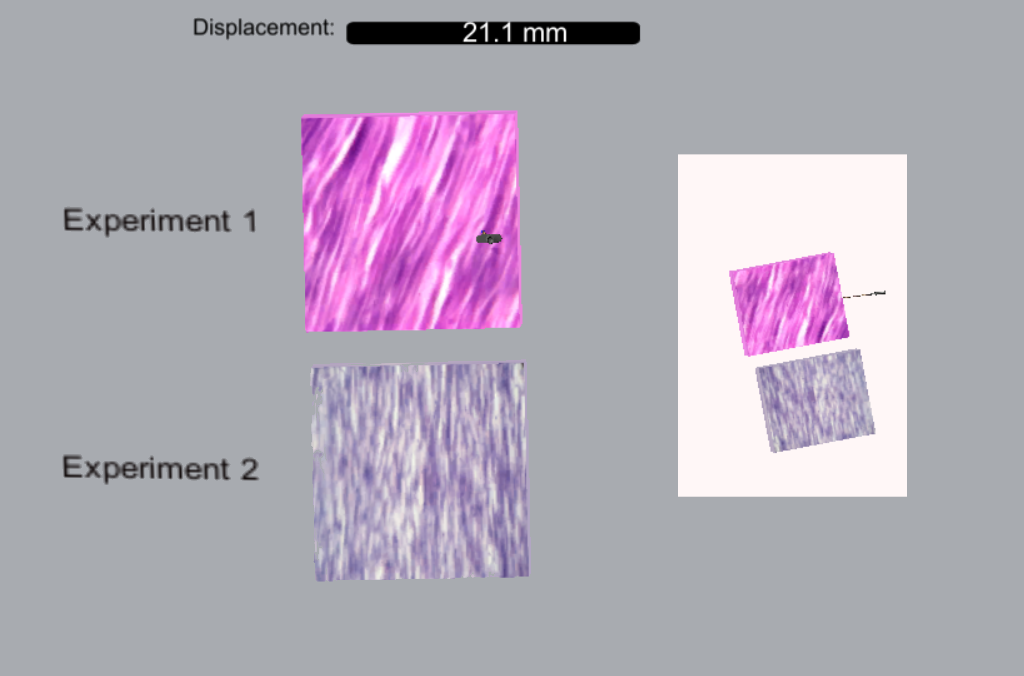
\includegraphics[width=0.8\linewidth]{capitulos/figuras/visual-experimentos.png} 
    \caption{Aparência visual dos experimentos 1 e 2. Na esquerda a vista de frente e na direita com fundo branco a vista lateral. As diferenças nas dimensões ocorrem somente na profundidade das camadas internas.}
    \label{fig:visualExperimentos1e2}
\end{figure}

\begin{figure}[ht!]
    \centering
        \begin{tabular}{cc}
        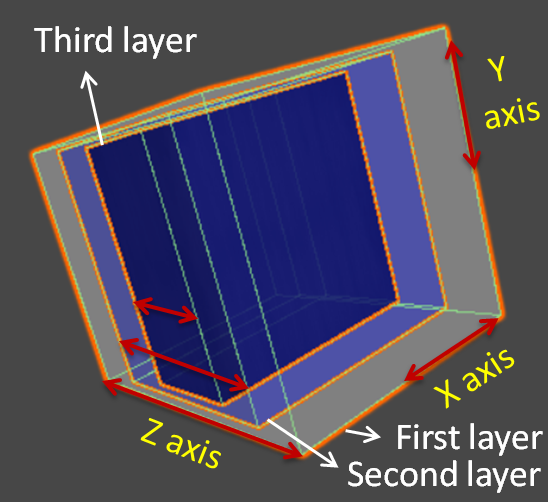
\includegraphics[width=0.3\linewidth]{capitulos/figuras/First.Experiment - axis.PNG} & 
        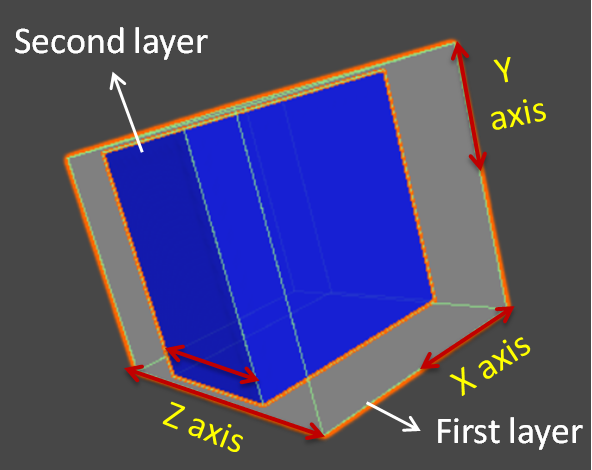
\includegraphics[width=0.35\linewidth]{capitulos/figuras/Second.Experiment - axis.PNG} 
        \\
        (a) & (b)
        \end{tabular}
    \caption{Os objetos 3D representam as camadas de cada experimento: (a) Primeiro experimento (b) Segundo experimento.}
    \label{fig:objectsExperiments}
\end{figure}

O tamanho da agulha é 65 milímetros (mm). Para os dois experimentos foi incluída uma deformação na interface de cada camada com o aumento da força antes da perfuração. Essa deformação é uma função da força necessária para perfurar cada camada. Foi usado um valor máximo de deformação de cinquenta vezes o valor da propriedade \textit{Pop through} em cada camada. O deslocamento desta deformação máxima é medido em milímetros. Logo após ser perfurado o tecido reassume a posição original (sem deformação). 

A Tabela \ref{tab:propHapticoPrimeiroExperimento} descreve os valores configurados nas propriedades de cada camada do primeiro experimento. A deformação máxima para a primeira camada é de 2,5 mm, que corresponde a cinquenta vezes 0,05 (\textit{Pop Through} da primeira camada). A Figura \ref{fig:forcaDeslocamentoExperimento1} apresenta um gráfico da força aplicada (eixo vertical) com o deslocamento da agulha representado no eixo horizontal para o experimento 1. As setas nesta imagem indicam a extensão da deformação de cada camada, começando na esquerda quando a agulha começa a tocar a camada e terminando na direita quando a camada é perfurada. O deslocamento da agulha observado na área sob as setas representa menores variações por conta da necessidade do aumento de força que vai deslocando lentamente a agulha enquanto deforma a camada até o momento em que a camada é perfurada. O espaço entre as setas da Figura \ref{fig:forcaDeslocamentoExperimento1} representa quando a agulha está em movimento dentro das camadas. 
As diferenças mais significativas no eixo de deslocamento da agulha (eixo X) podem ser observados nas áreas marcadas com retângulos. Estas áreas do gráfico representam o aumento da velocidade de deslocamento da agulha imediatamente após a perfuração de cada camada. Isto acontece por que imediatamente antes da perfuração da camada está sendo empregada uma força necessária para perfuração que, ao ser mantida após a perfuração, implica num maior deslocamento dentro da camada. Observa-se nos picos de força (eixo Y) que a força necessária para perfurar a camada é bastante superior a força necessária para movimentação da agulha dentro da camada. 

\begin{table}[!ht]
\begin{center}
\caption{Configurações das propriedade do \textit{plugin} do háptico usadas no primeiro experimento.}
\label{tab:propHapticoPrimeiroExperimento}
\begin{tabular}{|l|lll|}
\hline
\multicolumn{1}{|c|}{\multirow{2}{*}{Propriedade}} & \multicolumn{3}{c|}{Camada}  \\ \cline{2-4} 
\multicolumn{1}{|c|}{} & \multicolumn{1}{c|}{1} & \multicolumn{1}{c|}
{
\begin{tabular}[c]{@{}c@{}}2\end{tabular}} & \multicolumn{1}{c|}{\begin{tabular}[c]{@{}c@{}}3\end{tabular}}  \\ 
\hline\hline
\textit{Stiffness} & \multicolumn{1}{l|}{0,75} & \multicolumn{1}{l|}{0,75} & \multicolumn{1}{l|}{0,75} \\ 
\textit{Pop Through} & \multicolumn{1}{l|}{0,05} & \multicolumn{1}{l|}{0,15} & \multicolumn{1}{l|}{0,10}  \\ 
\textit{Punctured Static Friction} & \multicolumn{1}{l|}{0,20} & \multicolumn{1}{l|}{0,30} & \multicolumn{1}{l|}{0,30}  \\ 
\textit{Punctured Dynamic Friction} & \multicolumn{1}{l|}{0,30} & \multicolumn{1}{l|}{0,30} & \multicolumn{1}{l|}{0,10}  \\ 
\hline
\end{tabular}
\end{center}
\end{table}

O segundo experimento tem duas camadas e sua configuração é descrita na Tabela \ref{tab:propHapticoSegundoExperimento}. A curva de força versus deslocamento da agulha desse experimento está ilustrada na Figura \ref{fig:forcaDeslocamentoExperimento2} e aqui se aplicam as mesmas considerações feitas em relação as marcações de setas e retângulos discutidas em relação a Figura \ref{fig:forcaDeslocamentoExperimento1}.

O ponto de referência considerado para a interface da primeira camada em cada experimento foi 0 mm. Esta referência serve para medir o deslocamento da agulha a partir do toque na primeira camada até atingir todas as demais camadas. Esta medida é feita na direção ortogonal à superfície da camada tocada pelo usuário com a agulha virtual. A segunda camada do primeiro experimento está posicionada a 25 mm a partir desta referência e a terceira camada está a 50 mm. A segunda camada do segundo experimento inicia a 35mm do ponto de referência.

\begin{figure}[ht!]
    \centering
    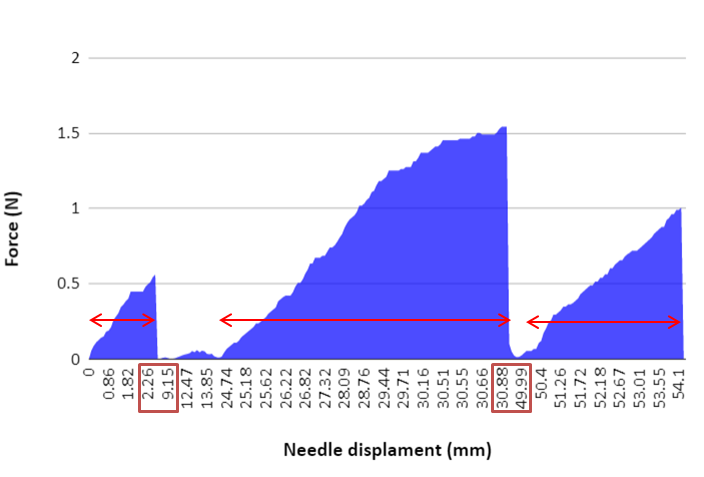
\includegraphics[width=0.8\linewidth]{capitulos/figuras/Experiment 1 - Force x Needle displacement - marked.PNG} 
    \caption{Relação entre força e o deslocamento da agulha média considerando dez simulações no experimento 1.}
    \label{fig:forcaDeslocamentoExperimento1}
\end{figure}

\begin{table}[!ht]
\begin{center}
\caption{Configurações das propriedade do \textit{plugin} do háptico usadas no segundo experimento.}
\label{tab:propHapticoSegundoExperimento}
\begin{tabular}{|l|ll|}
\hline
\multicolumn{1}{|c|}{\multirow{2}{*}{Propriedade}} & \multicolumn{2}{c|}{Camada}  \\ \cline{2-3} 
\multicolumn{1}{|c|}{} & \multicolumn{1}{c|}{1} & \multicolumn{1}{c|}{\begin{tabular}[c]{@{}c@{}}2\end{tabular}}  \\  
\hline\hline
\textit{Stiffness} & \multicolumn{1}{l|}{0,75} & \multicolumn{1}{l|}{0,20}  \\ 
\textit{Pop Through} & \multicolumn{1}{l|}{0,05} & \multicolumn{1}{l|}{0,15}  \\ 
\textit{Punctured Static Friction} & \multicolumn{1}{l|}{0,90} & \multicolumn{1}{l|}{0,10}  \\ 
\textit{Punctured Dynamic Friction} & \multicolumn{1}{l|}{0,20} & \multicolumn{1}{l|}{0,10}   \\ 
\hline
\end{tabular}
\end{center}
\end{table}

\begin{figure}[ht!]
    \centering
    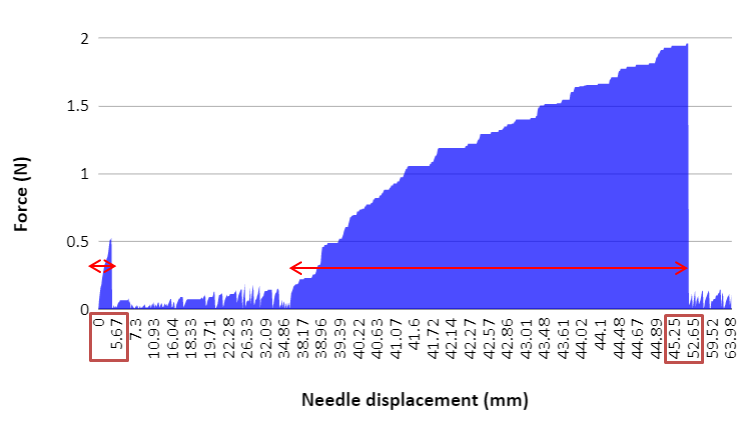
\includegraphics[width=0.8\linewidth]{capitulos/figuras/Experiment 2 - Force x Needle displacement - marked.PNG} 
    \caption{Relação entre força e o deslocamento da agulha da média de dez simulações no experimento 2.}
    \label{fig:forcaDeslocamentoExperimento2}
\end{figure}

A quantidade de camadas de cada experimento proposto aqui difere do número original de camadas do procedimento descrito na seção~\ref{sec:anestesiaRaquidiana}. Isto por que a ideia não foi representar todo o corpo ou procedimento. A ideia é reproduzir, nos experimentos, as sensações mais importantes e críticas envolvidas neste procedimento. As outras interfaces entre as camadas são simples reproduções de partes das que foram incluídas nestes experimentos.

\subsection{Questionário}
\label{sec:questionario}

Entre os testes com a ferramenta de nivelamento no uso do háptico e o início do experimento os questionários com as perguntas de cada experimento foram apresentados para os usuários. Isto foi feito de forma que durante o experimentos cada um pudesse coletar as informações necessárias para responder cada pergunta. Apresentamos a seguir as perguntas que foram apresentadas para os voluntários.

Questão 1) Experimentos número 1 e 2: Quantas camadas você pode sentir desde o momento de perfurar o objeto até chegar ao deslocamento máximo de 65mm? 
Observação: Cada camada é identificada por uma restrição a perfuração.

Questão 2) Experimento número 1: Ordene as camadas de forma decrescente em relação a resistência a perfuração.    
Exemplo de resposta: 1, 2 (considerando que existam duas camadas e a primeira é mais resistente que a segunda).

Questão 3) Experimento número 1: Em qual posição cada camada começa, ou seja, qual o ponto do deslocamento da agulha onde você identificou resistência para perfuração? 
Exemplo de resposta: Camada 1 = 0mm, Camada 2 = 10mm e Camada 3 = 30mm (considerando que tenham sido identificadas 3 camadas com resistências diferentes nestes 3 pontos de deslocamento).

Questão 4) Experimento número 2: Em qual intervalo (início e fim) de deslocamento foi observado a maior resistência ao movimento de perfuração? 
Exemplo de resposta: Entre 10mm e 20mm.

Questão 5) Experimento número 2: Em qual intervalo (início e fim) de deslocamento foi observado uma necessidade de aplicação de uma força constante para o deslocamento? 
Exemplo: Entre 10mm e 20mm.

Todas as perguntas envolvem aspectos de identificação tátil vitais na realização de uma raquianestesia. Os exemplos de resposta foram ilustrados com o intuito de facilitar a posterior análise das respostas procurando evitar excessos de descrições desnecessárias. A identificação do comportamento elástico é avaliado nas questões 1, 3 e 5 enquanto a questão 4 trata da identificação do comportamento plástico. A questão que envolve a identificação da posição inicial (3) assim como as que pedem a identificação de intervalos de comportamentos (4 e 5) sofrem impacto do deslocamento das interfaces de cada camada via deformação. Todas as camadas iniciam na sua posição de origem e apresentam um deslocamento por deformação imediatamente antes da perfuração que alteram esta posição. Para fins de avaliação, consideramos corretas as respostas entre o ponto inicial e o ponto final de deslocamento pela deformação nas identificações de interface de cada camada.  

\subsection{Respostas}
\label{sec:respostas}

Nesta seção apresentamos uma compilação das respostas dos participantes às perguntas de cada experimento. Para o primeiro
experimento, as respostas foram as seguintes:

Questão 1) Onze voluntários (aproximadamente 92\%) responderam corretamente.

Questão 2) Sete voluntários (58\%) responderam corretamente para todas as camadas. Onze voluntários (92\%) acertaram a camada menos resistente e nove (75\%) acertaram a mais resistente.

Questão 3) Nove voluntários (75\%) responderam corretamente para todas as camadas. Todos acertaram a segunda camada e onze voluntários (92\%) acertaram a primeira camada. 

Após responder o primeiro questionário as mesmas pessoas executaram o segundo experimento e responderam o questionário deste conforme descrito a seguir:

Questão 1) Todos os voluntários (100\%) responderam corretamente.

Questão 4) Nove voluntários (75\%) responderam corretamente.

Questão 5) Oito voluntários (aproximadamente 67\%) responderam corretamente. Nove (75\%) acertaram o início.

\subsection{Avaliação dos resultados}
\label{sec:avaliacao}

Nesta seção detalhamos cada um dos comportamentos mais importantes do procedimento coberto nestes experimentos que foram criados para avaliar a percepção do usuário sobre o comportamento das
camadas virtuais sendo perfuradas por uma agulha.

\subsubsection{Resistência à punção}

Considerando os sentimentos ou sensações de resistência à punção (o assunto da questão dois), apenas 58\% dos respondentes ordenaram corretamente todas as camadas de acordo com suas resistências. Este resultado indica a necessidade de se aumentar a diferença na força necessária para perfurar cada camada para permitir uma identificação mais facilitada de todas estas características. É importante ressaltar aqui que esta seria uma solução a ser considerada se o público alvo destes experimentos tivesse sido de anestesistas experientes fazendo a avaliação do sentimento tátil de cada camada em relação ao que estes vivenciam nos procedimentos pacientes reais. Na mesma pergunta, um número maior de voluntários identificaram a camada mais resistente ou a menos resistente à perfuração. Essa identificação é essencial para indicar quando a agulha penetra no ligamento amarelo (tecido mais resistente) ou a dura-máter (tecido menos resistente). Como estas duas camadas estão posicionadas no corpo humano uma após a outra (considerando o ângulo de perfuração correto), a correta identificação de uma é, por si só, um passo essencial na simulação correta do procedimento de raquianestesia.

\subsubsection{Comportamento elástico}

Quanto à identificação do comportamento elástico (questões 1, 3 e 5), apenas a questão cinco recebeu pontuação inferior a 75\%. No entanto, mesmo nesta questão, apenas três voluntários apontaram erroneamente o ponto de partida do intervalo com maior restrição ao movimento da agulha, ou seja, 75\% acertaram onde esta camada começa. Considerando somente os participantes que acertaram o ponto de partida apenas um deles identificou erroneamente o ponto final desta camada. 

Tivemos ótimas respostas na detecção do número de camadas (questão um) em todos experimentos. Identificar as camadas penetradas é uma das partes mais críticas do procedimento de raquianestesia. Isto indica tanto a determinação correta da sensação de \textit{popping} da interface entre as camadas e reconhecimento do comportamento elástico que ocorre imediatamente antes de perfurar cada camada.

Quanto à identificação do ponto de início de cada camada (questão três) também é importante destacar o número de casos corretamente identificados (75\%). Esta resposta reforça a necessidade de utilização de valores de profundidade desde a pele até o espaço subaracnóide próximo da realidade para treinar melhor os anestesistas. Cada ponto de partida da camada está relacionado com o início do comportamento elástico e é necessário aumentar a força para prosseguir com o avanço da agulha em cada interface entre camadas. 

\subsubsection{Comportamento plástico}

A questão quatro, com 75\% de sucesso na identificação, aborda um outro comportamento de grande importância na raquianestesia. A identificação de estar no interior da camada que apresenta a maior
resistência, ou seja, sentir uma força de resistência constante contra o movimento através da camada (comportamento plástico), está relacionado ao ligamento amarelo, que ocorre imediatamente antes de se atingir o espaço peridural. As respostas a esta pergunta
confirmam que esse comportamento pode ser simulado adequadamente.

\section{Testes de usabilidade}
\label{sec:testeUsabilidade}

Esta seção detalha os testes para avaliação da usabilidade do ambiente de simulação desenvolvido nesta tese. Para isto foi feita uma pequena simplificação no que diz respeito a execução do procedimento de raquianestesia usando o dispositivo háptico. Isto foi feito uma vez que a intenção nesta fase era a de se avaliar a usabilidade por pessoas não especialistas na execução do procedimento de raquianestesia. Com isso a colisão referente aos toques das agulhas nas vértebras dos pacientes simulados foi removida para este teste fazendo que a execução do procedimento pudesse ser feita de forma mais simples e sem necessidade de conhecimento médico de anestesistas. Esta simplificação foi feita através da remoção da \textit{Tag Touchable} do objeto do modelo 3D que representa as vértebras. 
A ideia com isto foi a de não frustrar os voluntários dos testes mesmo que previamente informando a eles que o desempenho deles em relação a correta execução do procedimento não estava em avaliação. Particularmente esta decisão se demonstrou ter sido acertada uma vez que alguns voluntários mesmo com essa simplificação aparentavam alguma frustração quando tinham dificuldade na execução do procedimento até o final e quando recebiam notas baixas pela sua execução. Importante ressaltar que todos os voluntários foram orientados que não era necessário executar corretamente o procedimento uma vez que eles não possuíam o conhecimento necessário para tal. Todos os testes foram efetuados nas dependências do instituto de computação da Universidade Federal Fluminense com participação de alunos de graduação, mestrado e doutorado.

O ambiente de treinamento simplificado foi apresentado a sessenta e dois voluntários que fizeram uso do equipamento háptico, todos estes voluntários eram estudantes de ciência da computação com idades variando entre 18 e 58 anos sendo cinquenta homens e doze mulheres. Todos os voluntários concordaram com o termo de consentimento de participação nesta pesquisa e receberam uma breve explicação (cinco minutos) a respeito do procedimento de uso do equipamento háptico e do propósito do sistema. Em seguida usaram o ambiente de treinamento para execução de ao menos um procedimento de raquianestesia. A montagem do equipamento foi feita conforme ilustrado na Figura~\ref{fig:montagemTesteUsabilidade} e só teve uma pequena variação com alternância do lado do dispositivo háptico quando o voluntário era canhoto.

\begin{figure}[ht!]
    \centering
    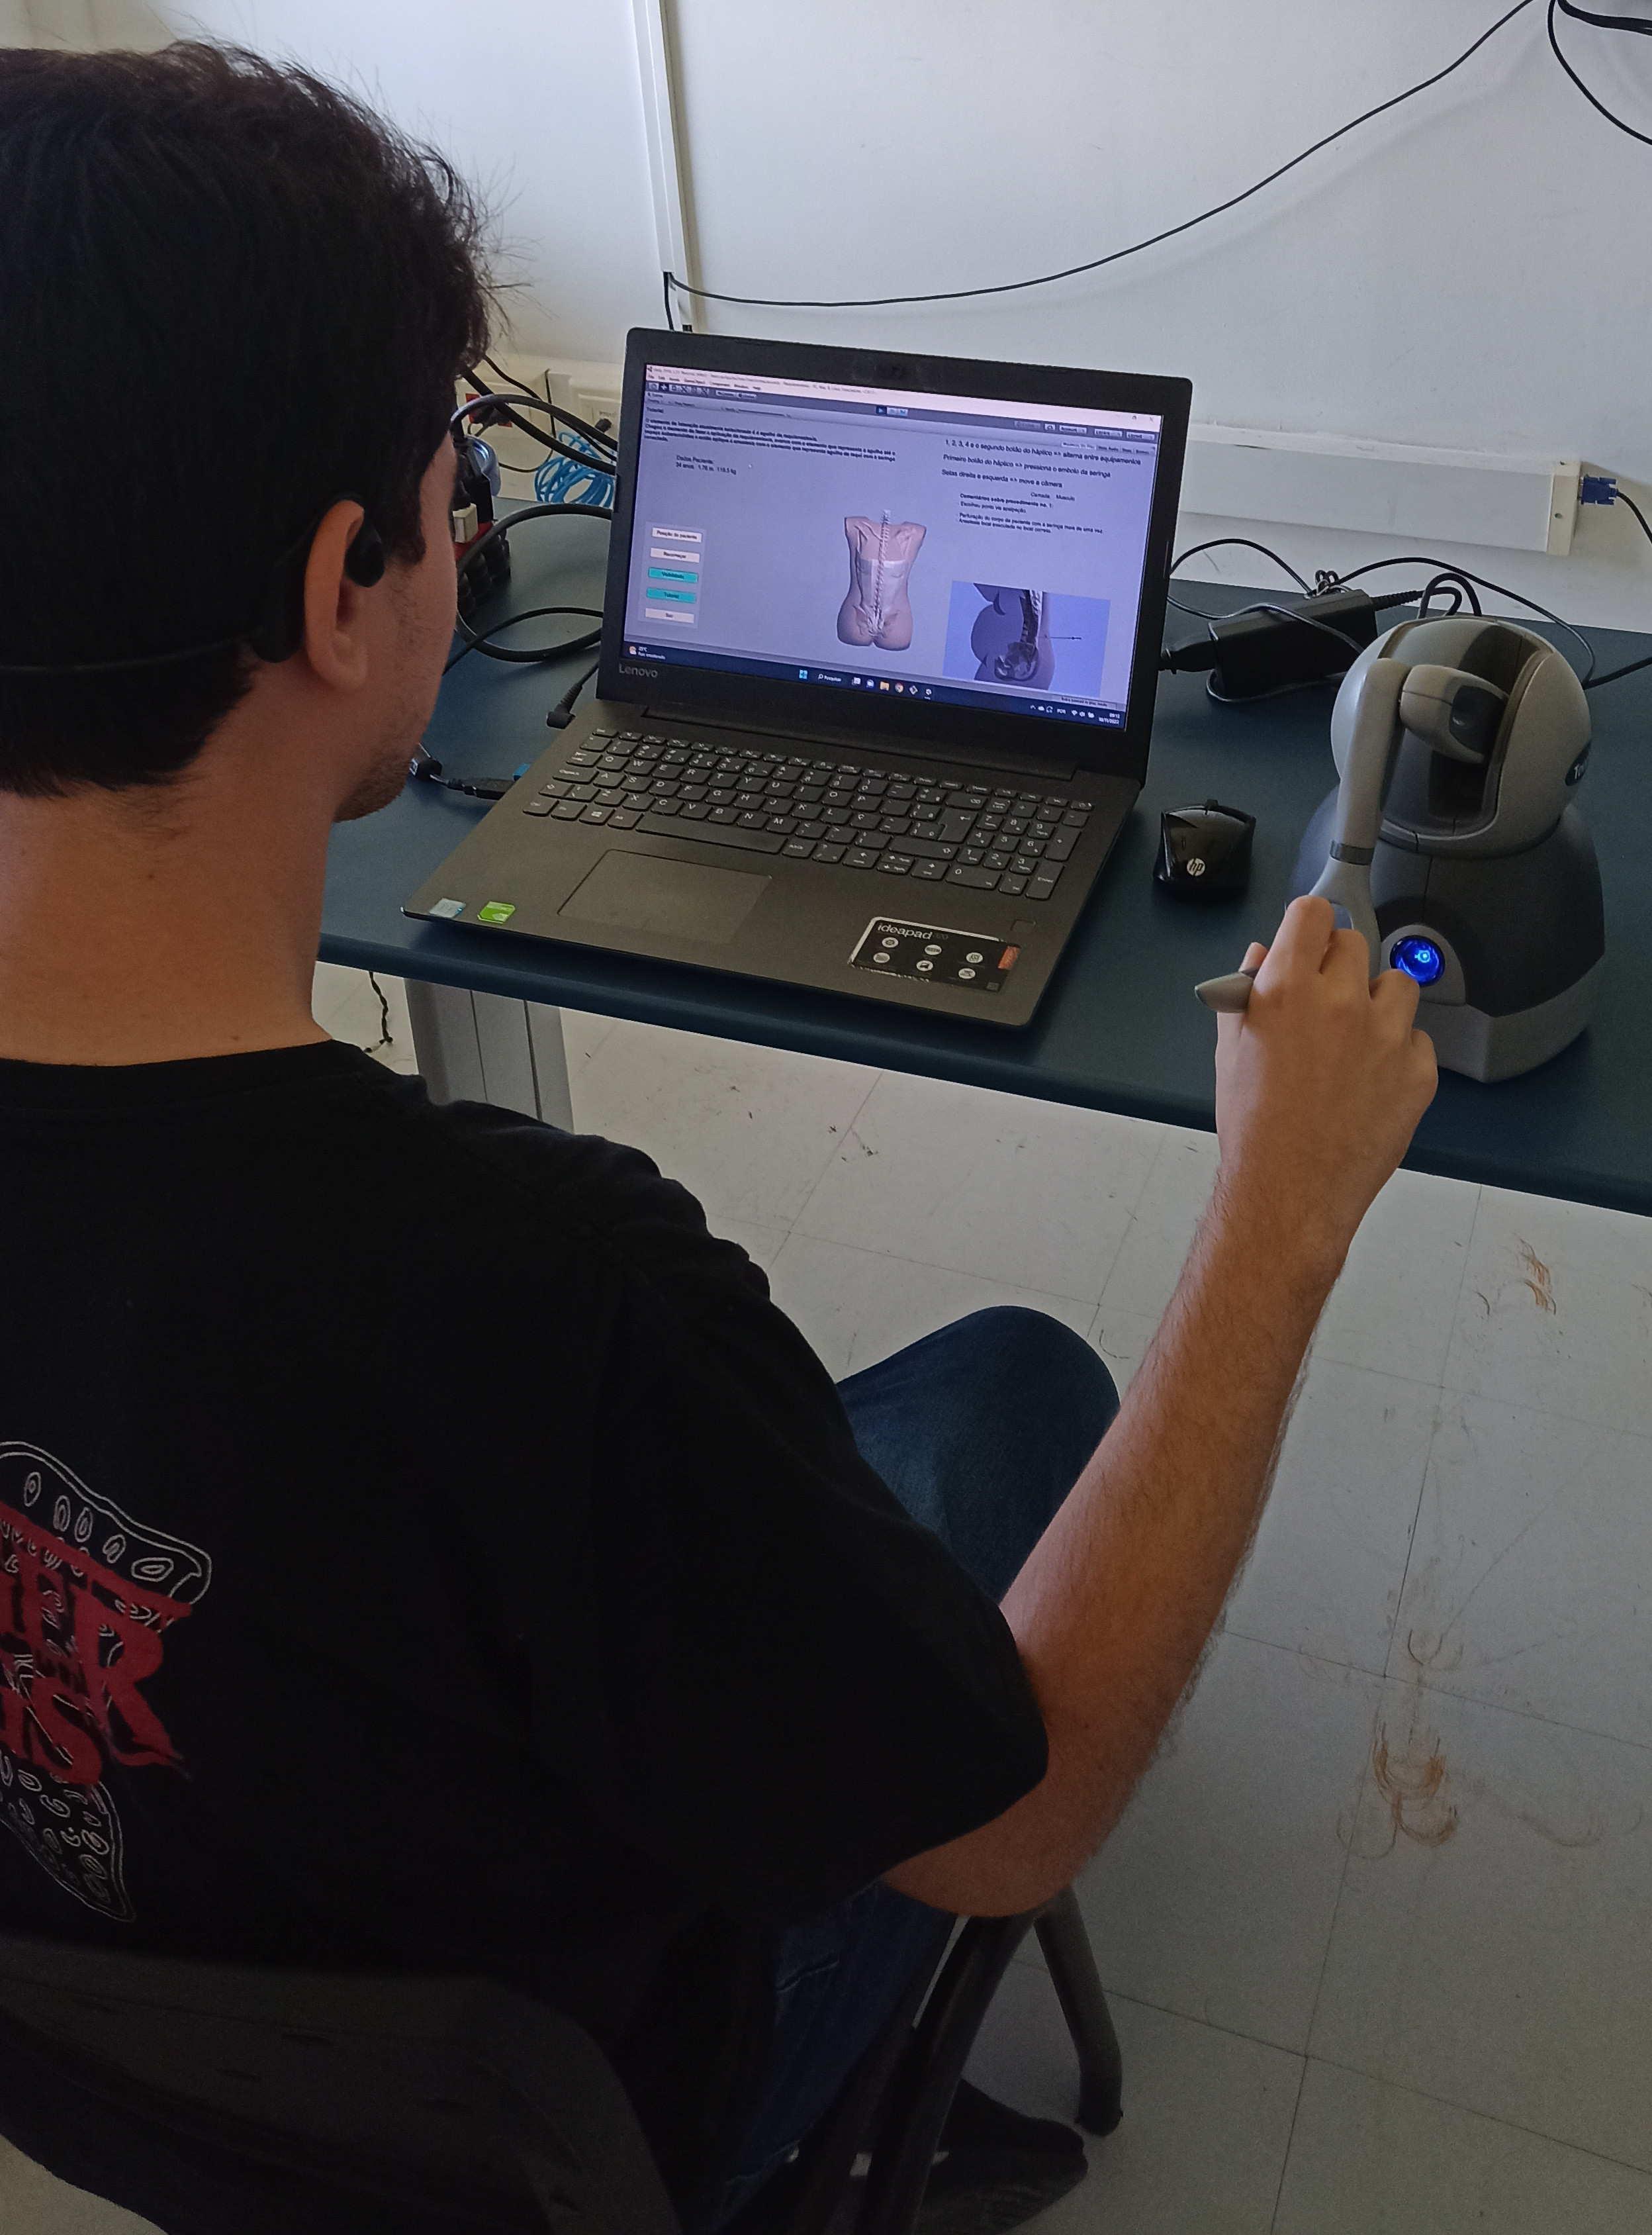
\includegraphics[width=0.4\linewidth]{capitulos/figuras/montagem-teste-usabilidade.jpg} 
    \caption{Montagem do ambiente de treinamento em uso durante os testes de usabilidade.}
    \label{fig:montagemTesteUsabilidade}
\end{figure}

\subsection{Questionário}
\label{sec:questionarioUsabilidade}

Após a execução dos procedimentos por cada voluntário usando o ambiente de simulação para treinamento simplificado um questionário foi apresentado para os usuários. As perguntas apresentadas para os voluntários estão descritas a seguir. As respostas foram coletadas em sua maioria (de um a onze) usando a escala \textit{likert} variando de 1 (Discordo fortemente) até 5 (Concordo fortemente). As dez primeiras perguntas foram feitas baseadas no método \textit{\acrfull{SUS}} \cite{Brooke2013} criado em 1986 para uma avaliação quantitativa da usabilidade. Ele é um método muito conhecido e utilizado e propõe uma escala numérica para avaliar a: Efetividade (se os usuários conseguem completar seus objetivos); 
Eficiência (o esforço e recursos que são necessários para completar os objetivos); e
Satisfação (em relação a experiência do uso do ambiente proposto aqui). A décima primeira pergunta foi incluída para ter um retorno a respeito do modo tutorial desenvolvido no sistema. A décima segunda questão foi uma pergunta pra resposta textual a respeito de sugestões de possíveis melhorias.

\subsection{Respostas}
\label{sec:respostasUsabilidade}

Nesta seção apresentamos uma compilação das respostas dos participantes às perguntas do questionário.

Questão 1) Eu usaria esse sistema com frequência.

Questão 2) Eu acho o sistema desnecessariamente complexo.

Questão 3) Eu achei o sistema fácil de usar.

Questão 4) Eu acho que precisaria de ajuda de uma pessoa com conhecimentos técnicos para usar o sistema.

Questão 5) Eu acho que as várias funções do sistema estão muito bem integradas.

Questão 6) Eu acho que o sistema apresenta muita inconsistência.

Questão 7) Eu imagino que as pessoas aprenderão como usar esse sistema rapidamente.

Questão 8) Eu achei o sistema atrapalhado de usar.

Questão 9) Eu me senti confiante ao usar o sistema.

Questão 10) Eu precisei aprender várias coisas novas antes de conseguir usar o sistema.

Questão 11) O \textit{feedback} do modo tutorial esclarece dúvidas sobre a sequência de ações a ser executada.

Questão 12) Você tem alguma sugestão de alterações na interface que poderiam melhorar a usabilidade? Se sim, comente.

\subsection{Avaliação dos resultados}
\label{sec:avaliacaoUsabilidde}

Em relação as dez perguntas do \acrshort{SUS} a nota calculada a partir das respostas foi 76,9 o que de acordo com \textcite{BangorAaron2009} classifica o ambiente como ``Bom'' numa escalada que vai desde a ``Pior usabilidade imaginável'' pra uma nota a partir de 12,5 com 13,1 de desvio padrão até ``Melhor usabilidade imaginável'' para média 90,9 com 13,4 de desvio padrão. 
Quanto a avaliação do modo tutorial (questão 11) 69,4\% (43 voluntários) classificaram ele com o valor 4 ou 5 (Concordo fortemente). A distribuição destas respostas pode ser observada na Tabela~\ref{tab:tabelaRespostasModoTutorial}. As melhores sugestões apontadas em resposta a questão 12 foram incluídas na seção \ref{sec:trabFuturo}.

\begin{table}[!ht]
\begin{center}
\caption{Distribuição das respostas da questão 11.}
\label{tab:tabelaRespostasModoTutorial}
\begin{tabular}{|p{0.35\linewidth}|p{0.15\linewidth}|p{0.35\linewidth}|}
\hline
\textbf{Respostas da questão 11} & \textbf{Frequência} & \textbf{Frequência percentual (\%)}\\
\hline\hline
1 & 2 & 3,23\%\\
2 & 8 & 12,90\%\\
3 & 9 & 14,52\%\\
4 & 23 & 37,10\%\\
5 & 20 & 32,26\%\\
\hline
\end{tabular}
\end{center}
\end{table}

\section{Avaliações com especialistas}
\label{sec:testeEspecialistas}

Esta seção detalha as avaliações do ambiente de treinamento completo desenvolvido nesta tese por especialistas. Para possibilitar uma maior adesão, todos os testes com especialistas foram feitos nas dependências do Hospital Universitário Antônio Pedro, na secretaria do centro cirúrgico, com anuência de todos os responsáveis.

O ambiente de treinamento simplificado foi apresentado a dez voluntários que fizeram uso do equipamento háptico, nove destes voluntários eram anestesistas e um era residente de anestesia com idades variando entre 35 e 54 anos sendo cinco homens e cinco mulheres. Cinco tinham três anos ou menos de experiência em anestesia raquidiana, três tinham por volta de dez anos de experiência e dois deles tinham vinte dois anos com este tipo de anestesia. A frequência mensal de execução deste procedimento entre os voluntários variou entre seis e vinte procedimentos em média. Todos os voluntários concordaram com o termo de consentimento de participação nesta pesquisa e receberam uma breve explicação (de aproximadamente cinco minutos) a respeito do procedimento de uso do equipamento háptico e do propósito do sistema. Em seguida usaram o ambiente de treinamento para execução de ao menos um procedimento de raquianestesia. 

É importante ressaltar aqui que foi feita uma montagem inicial para execução dos procedimentos como na Figura~\ref{fig:montagemTesteUsabilidade}, porém alguns especialistas questionaram esta montagem por informarem que aquela posição não é a que eles tem o costume de executar o procedimento. Com isto adaptamos a montagem às posições preferidas de cada voluntário que fez este questionamento procurando se aproximar ao máximo do posição real de execução deles. As Figuras~\ref{fig:montagemTesteEspecialistasInicial} e \ref{fig:montagemTesteEspecialistas2e3} são exemplos das montagem que fizemos para execução dos procedimentos pelos especialistas. Na Figura~\ref{fig:montagemTesteEspecialistasInicial} está a nossa sugestão inicial, a Figura~\ref{fig:montagemTesteEspecialistas2e3} (a) mostra montagem de acordo com a preferência da voluntária em executar o procedimento de pé e a Figura~\ref{fig:montagemTesteEspecialistas2e3} (b) ilustra a montagem sugerida pelo voluntário para posicionamento do equipamento háptico que simula a agulha em frente ao ambiente virtual que simula o paciente.

\begin{figure}[ht!]
    \centering
    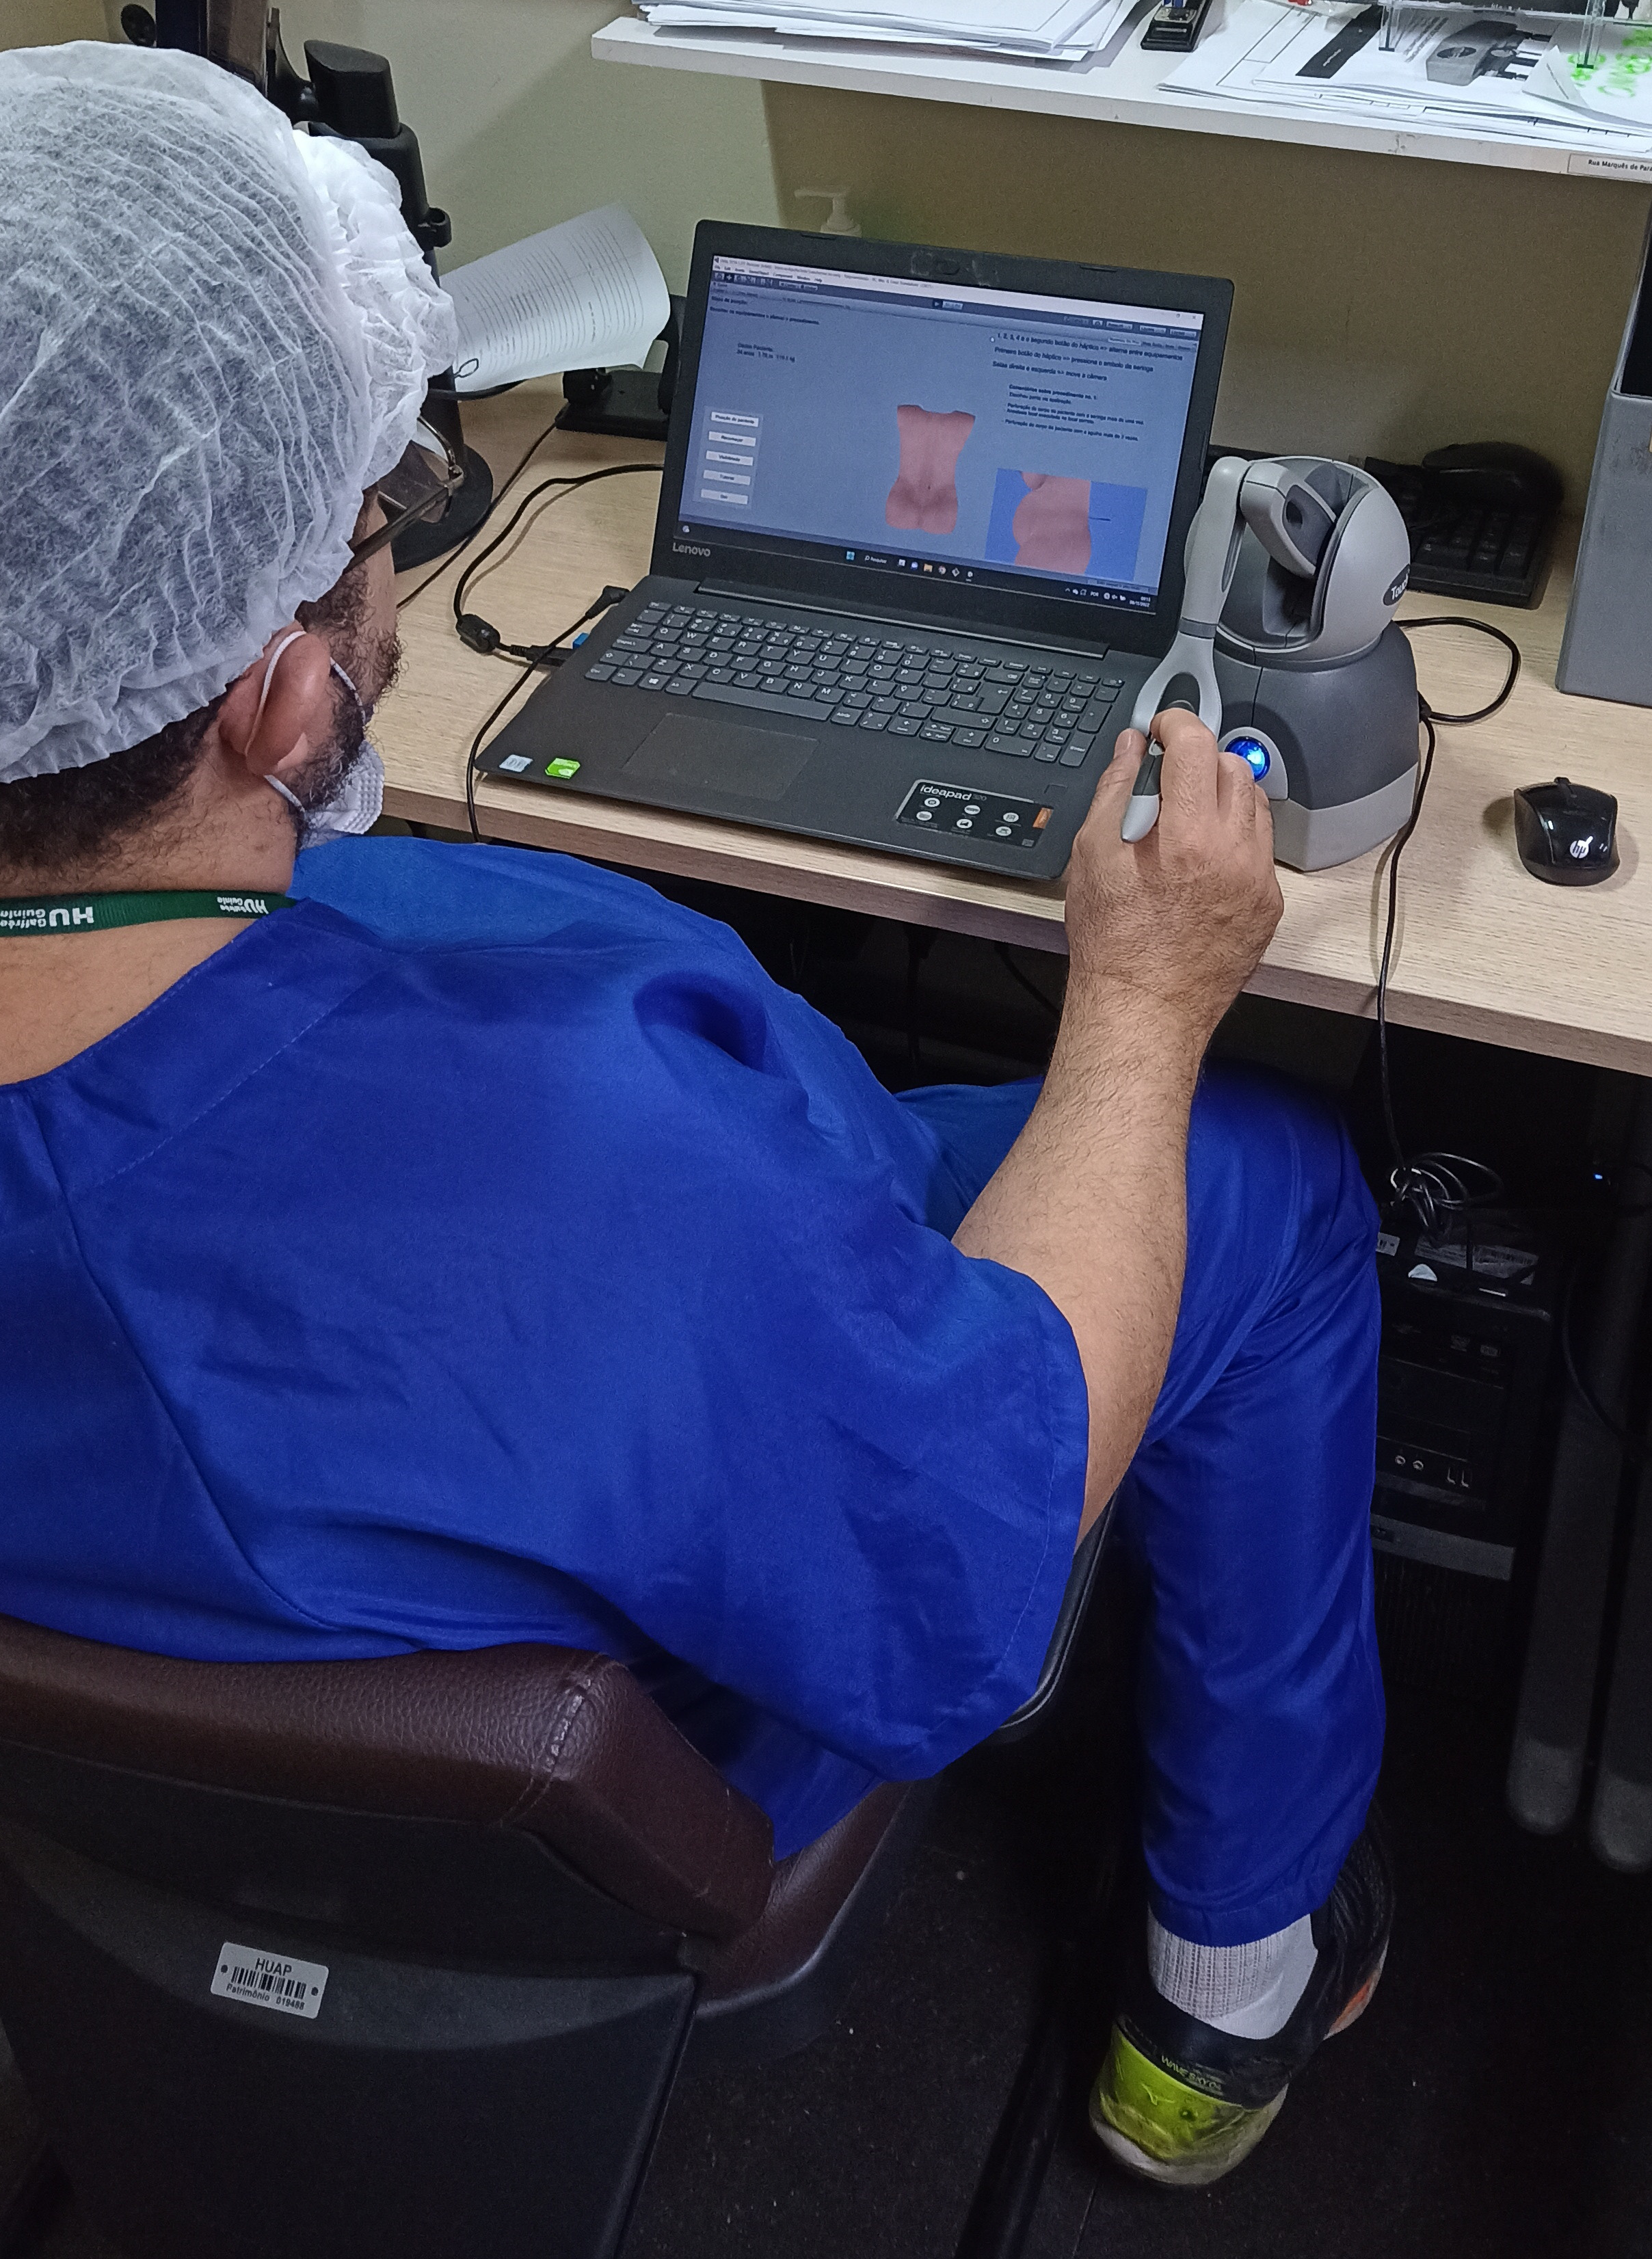
\includegraphics[width=0.4\linewidth]{capitulos/figuras/montagem-teste-especialistas-1.jpg} 
    \caption{Montagem do ambiente de treinamento em uso durante as avaliações com especialistas na posição sugerida inicial.}
    \label{fig:montagemTesteEspecialistasInicial}
\end{figure}

\begin{figure}[ht!]
    \centering
        \begin{tabular}{cc}
        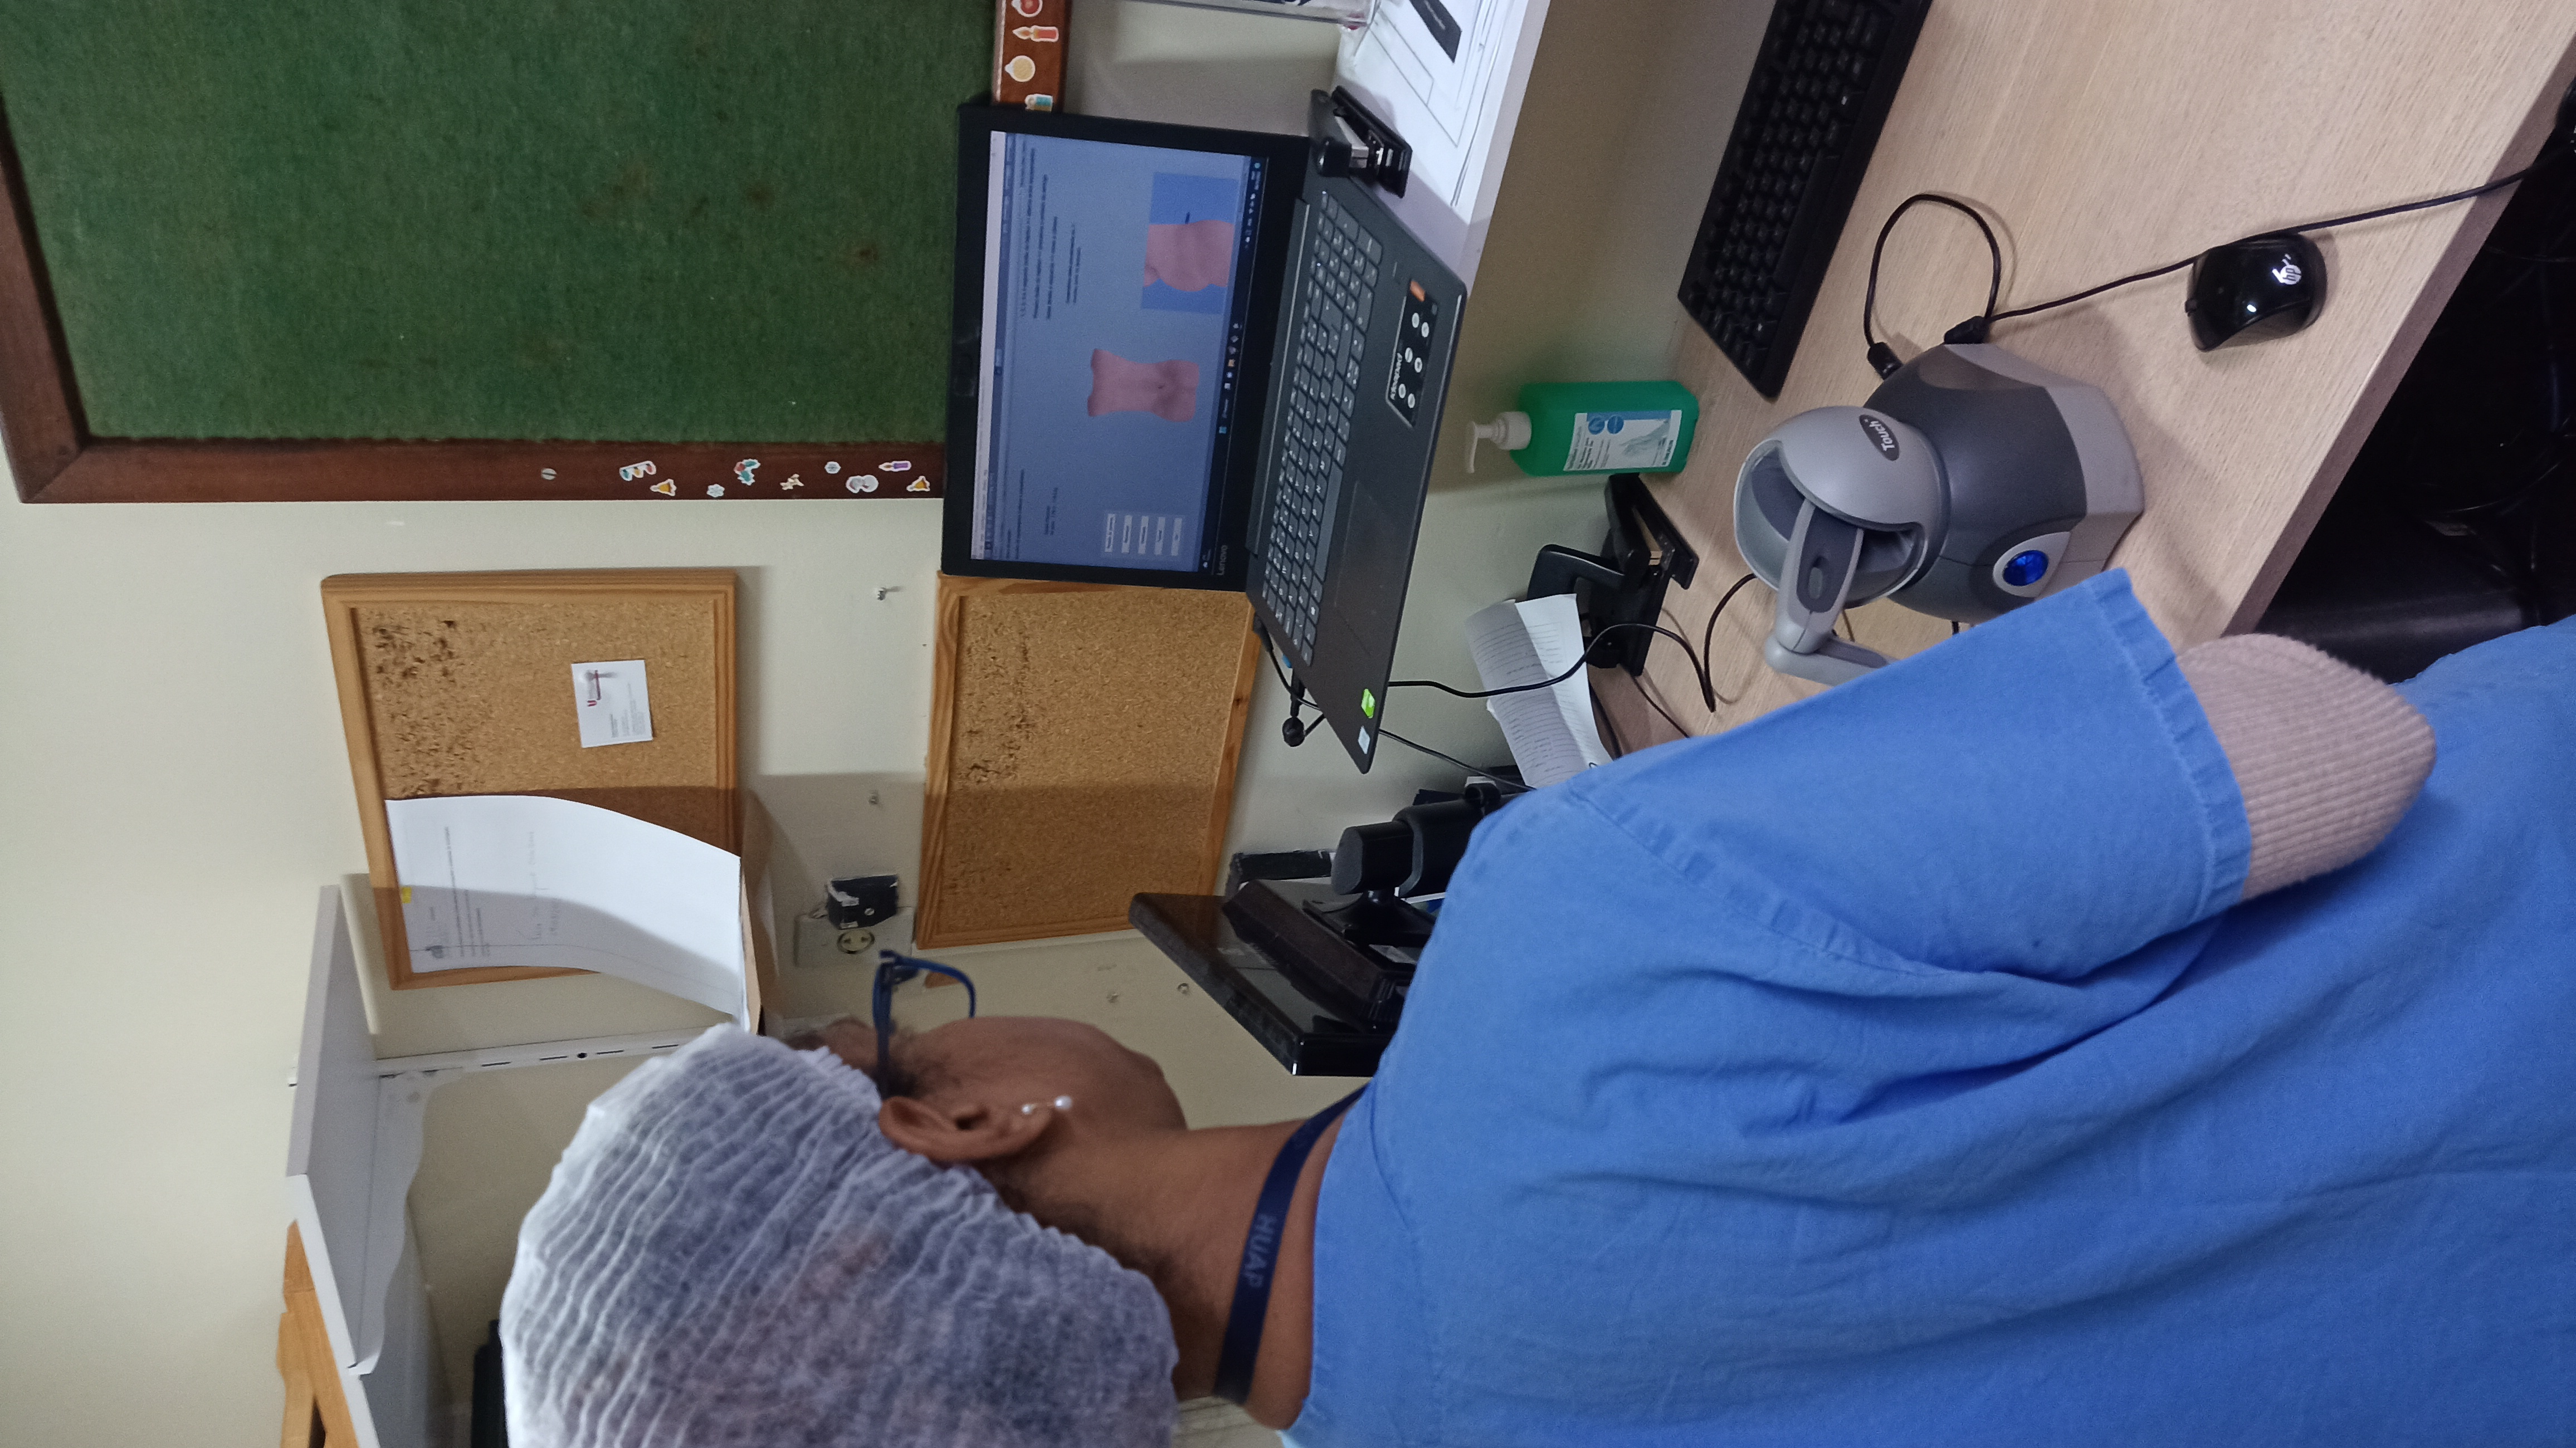
\includegraphics[angle=270,width=0.4\linewidth]{capitulos/figuras/montagem-teste-especialistas-2.jpg} & 
        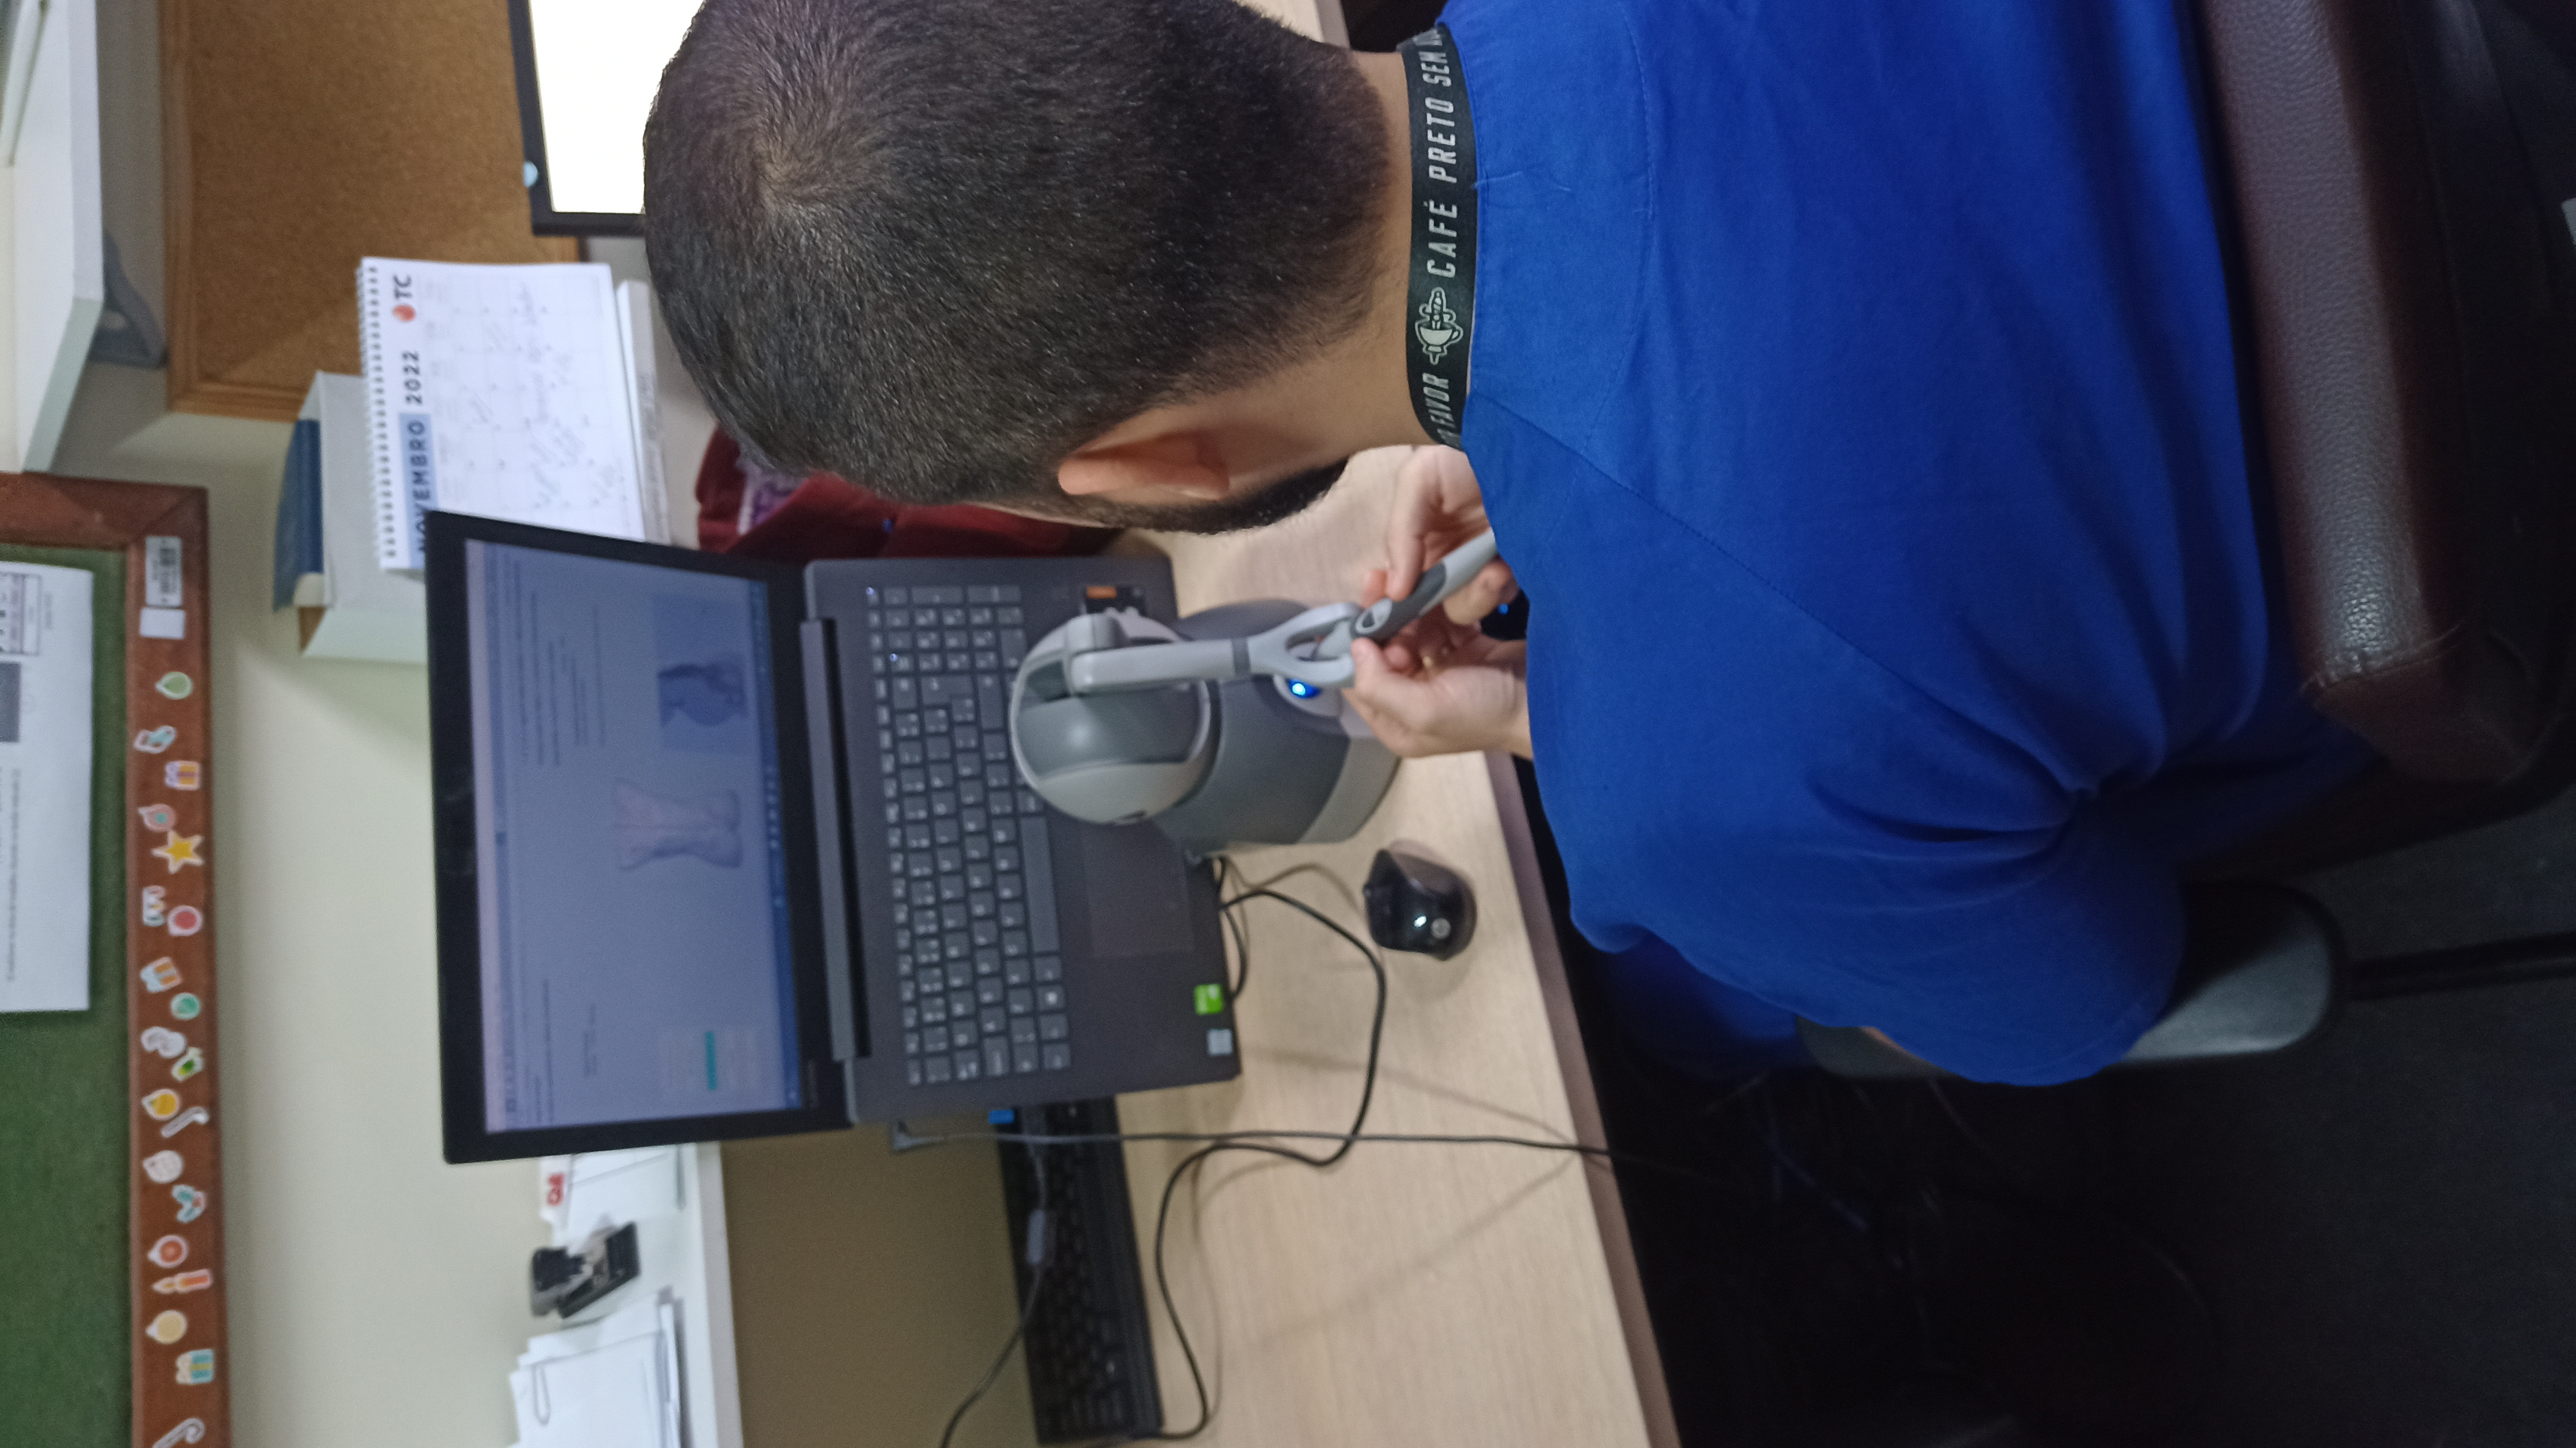
\includegraphics[angle=270,width=0.4\linewidth]{capitulos/figuras/montagem-teste-especialistas-3.jpg} 
        \\
        (a) & (b)
        \end{tabular}
    \caption{Montagem do ambiente de treinamento em uso durante as avaliações com especialistas com posicionamento adaptado a preferência dos voluntários: (a) Para uso em pé (b) Com dispositivo háptico a frente do computador simulando a agulha em frente ao paciente.}
    \label{fig:montagemTesteEspecialistas2e3}
\end{figure}

\subsection{Questionário}
\label{sec:questionarioEspecialistas}

Após a execução dos procedimentos por cada voluntário usando o ambiente de simulação para treinamento um questionário foi apresentado para os usuários. Apresentamos a seguir as perguntas que foram apresentadas para os voluntários. As respostas foram coletadas em sua maioria (de um a dez) usando a escala \textit{likert} variando de 1 (Concordo fortemente) até 6 (Discordo fortemente). Esta escala foi feita de forma contrária ao questionário de usabilidade pra fazer uma comparação direta com outro simulador \cite{Farber2009} do qual utilizamos algumas das perguntas feitas na avaliação deste já que os dois simuladores possuem algumas similaridades. A décima primeira questão foi uma tentativa de obter um retorno dos especialistas para melhorar o sistema de pontuação automático da qualidade da execução dos procedimentos.

Questão 1) A apalpação para descoberta do ponto de inserção da agulha traz ganhos no treinamento da sensação háptica?

Questão 2) As opções de posicionamento da paciente (sentada e deitada) atendem as necessidades do treinamento da raquianestesia?

Questão 3) As informações sobre o procedimento no modo tutorial deixam claro como usar o simulador para atingir os objetivos nos procedimentos?

Questão 4) O \textit{feedback} dado para o usuário durante e ao final dos procedimentos via textos explicativos é suficiente para promover uma evolução no treinamento?

Questão 5) Eu pude sentir forças diferentes nos diferentes tecidos virtuais?

Questão 6) O controle dos elementos de interação (dedo para apalpação, seringa e agulha) com o dispositivo háptico foi intuitivo?

Questão 7) A exibição dos pacientes virtuais parecia realista?

Questão 8) Os diferentes ângulos de visualização e transparência ajudaram a compreender a anatomia da região lombar?

Questão 9) Após o uso desta ferramenta num treinamento eu me sentiria mais confiante para realizar anestesia raquidiana do que sem este treinamento?

Questão 10) Considero útil o treinamento neste ambiente?

Questão 11) A pontuação atribuída a cada execução de procedimento inicia de zero e é somado um valor negativo para cada ação executada erradamente ou não executada e somado um valor positivo para cada ação executada corretamente. A seguir a tabela para cada ação. Na sequência coloquei os dados da Tabela~\ref{tab:PontosNotaProcedimento} e informei as seguintes características da pontuação:

A avaliação de desempenho através de pontuação de etapas tem como características:
\begin{itemize}
   \item Pontuação máxima = 10
   \item Pontuação mínima = -9
   \item Média das notas para desempenho satisfatório = 6
   \item Número mínimo de procedimentos = 3
 \end{itemize}

A última parte da questão 11 continha a seguinte pergunta:
``Você sugere uma mudança na forma de atribuição da pontuação dando mais ou menos peso para os itens atualmente configurados ou ainda sugere a inclusão de outros itens importantes que contribuam positivamente ou negativamente na pontuação? Em caso positivo comente:''

\subsection{Respostas}
\label{sec:respostasEspecialistas}

Nesta seção apresentamos uma compilação das respostas dos participantes às perguntas do questionário. Na Tabela~\ref{tab:comparacaoRespostasFarber} está o comparativo das respostas dos especialistas obtidas pelo estudo feito por \textcite{Farber2009} e o nosso estudo. O restante das respostas ao questionário que apresentamos para os voluntários onde utilizamos a mesma escala está detalhado na Tabela~\ref{tab:demaisRespotasQuestionarioEspecialistas}.

\begin{table}[!ht]
\begin{center}
\caption{Comparativo das respostas às questões similares coletadas para o nosso ambiente de simulação e o simulador de \textcite{Farber2009}, média (desvio padrão).}
\label{tab:comparacaoRespostasFarber}
\begin{tabular}{|ll|ll|}
\hline
\multicolumn{2}{|c|}{\begin{tabular}[c]{@{}c@{}}Ambiente de simulação \\ desenvolvido nesta Tese\\ (n=10)\end{tabular}} & \multicolumn{2}{c|}{\begin{tabular}[c]{@{}c@{}}Simulador de punção lombar de Färber\\ \cite{Farber2009}\\ (n=42)\end{tabular}}\\
\hline
\multicolumn{1}{|c|}{\begin{tabular}[c]{@{}c@{}}Número da questão\end{tabular}} & \multicolumn{1}{c|}{\begin{tabular}[c]{@{}c@{}}Resposta\end{tabular}} & \multicolumn{1}{|c|}{\begin{tabular}[c]{@{}c@{}}Número da questão\end{tabular}} & \multicolumn{1}{c|}{\begin{tabular}[c]{@{}c@{}}Resposta\end{tabular}} \\  %
\hline\hline
\multicolumn{1}{|c|}{\begin{tabular}[c]{@{}c@{}}5\end{tabular}} & \multicolumn{1}{c|}{\begin{tabular}[c]{@{}c@{}}2,8 (1,7)\end{tabular}} & \multicolumn{1}{c|}{\begin{tabular}[c]{@{}c@{}}2\end{tabular}} & \multicolumn{1}{c|}{\begin{tabular}[c]{@{}c@{}}1,5 (0,7)\end{tabular}} \\

\multicolumn{1}{|c|}{\begin{tabular}[c]{@{}c@{}}6\end{tabular}} & \multicolumn{1}{c|}{\begin{tabular}[c]{@{}c@{}}2,7 (1,3)\end{tabular}} & \multicolumn{1}{|c|}{\begin{tabular}[c]{@{}c@{}}3\end{tabular}} & \multicolumn{1}{c|}{\begin{tabular}[c]{@{}c@{}}2,2 (1,1)\end{tabular}} \\

\multicolumn{1}{|c|}{\begin{tabular}[c]{@{}c@{}}7\end{tabular}} & \multicolumn{1}{c|}{\begin{tabular}[c]{@{}c@{}}3,3 (1,3)\end{tabular}} & \multicolumn{1}{|c|}{\begin{tabular}[c]{@{}c@{}}5\end{tabular}} & \multicolumn{1}{c|}{\begin{tabular}[c]{@{}c@{}}2,0 (1,1)\end{tabular}} \\

\multicolumn{1}{|c|}{\begin{tabular}[c]{@{}c@{}}8\end{tabular}} & \multicolumn{1}{c|}{\begin{tabular}[c]{@{}c@{}}3,2 (1,4)\end{tabular}} & \multicolumn{1}{|c|}{\begin{tabular}[c]{@{}c@{}}6\end{tabular}} & \multicolumn{1}{c|}{\begin{tabular}[c]{@{}c@{}}1,6 (0,7)\end{tabular}} \\

\multicolumn{1}{|c|}{\begin{tabular}[c]{@{}c@{}}9\end{tabular}} & \multicolumn{1}{c|}{\begin{tabular}[c]{@{}c@{}}3,9 (1,5)\end{tabular}} & \multicolumn{1}{|c|}{\begin{tabular}[c]{@{}c@{}}7\end{tabular}} & \multicolumn{1}{c|}{\begin{tabular}[c]{@{}c@{}}1,9 (1,1)\end{tabular}} \\

\multicolumn{1}{|c|}{\begin{tabular}[c]{@{}c@{}}10\end{tabular}} & \multicolumn{1}{c|}{\begin{tabular}[c]{@{}c@{}}2,3 (1,2)\end{tabular}} & \multicolumn{1}{|c|}{\begin{tabular}[c]{@{}c@{}}8\end{tabular}} & \multicolumn{1}{c|}{\begin{tabular}[c]{@{}c@{}}1,5 (0,7)\end{tabular}} \\

\hline
\end{tabular}
\end{center}
\end{table}

\begin{table}[!ht]
\begin{center}
\caption{Média e desvio padrão das demais respostas ao questionário apresentado aos especialistas em relação ao ambiente de simulação desenvolvido nesta tese.}
\label{tab:demaisRespotasQuestionarioEspecialistas}
\begin{tabular}{|p{0.35\linewidth}|p{0.15\linewidth}|p{0.35\linewidth}|}
\hline
\textbf{Número da questão} & \textbf{Média} & \textbf{Desvio padrão}\\
\hline\hline
1 & 2,6 & 1,2\\
2 & 1,9 & 1,4\\
3 & 2,3 & 1,4\\
4 & 2,5 & 1,3\\
\hline
\end{tabular}
\end{center}
\end{table} 

A maioria dos especialistas fez comentários sobre possíveis melhorias para o ambiente de simulação no lugar de responder textualmente a questão 11. A única resposta a respeito de melhoria na pontuação foi a de aumentar o peso negativo do item ``Avanço com a seringa até camadas indevidas (ex. ossos, espaço epidural)''. Seguem a lista de comentários dos especialistas que foram feitos de forma oral: 
\begin{itemize}
   \item Inclusão da informação a respeito da angulação da agulha a cada instante;
   \item É necessário melhorar a curvatura do corpo;
   \item A visibilidade da agulha fica ruim em alguns instantes e é complicado fazer o acompanhamento das duas telas (vista traseira e lateral);
   \item Importância do uso de óculos 3D pra melhorar a imersão;
   \item Dificuldade em ver a ponta da agulha;
   \item Falta de contraste entre agulha e paciente;
   \item O ideal seria que quando a agulha estivesse perfurando as camadas fosse dado um zoom na visão lateral.
 \end{itemize}

\subsection{Avaliação dos resultados}
\label{sec:avaliacaoEspecialistas}

É importante ressaltar que apesar do ambiente de simulação desta tese e o simulador de punção lombar de Färber \cite{Farber2009} possuírem similaridades o protocolo utilizado e diversas características dos testes foram consideravelmente diferente nos dois casos. A população utilizada nesta tese foi de dez médicos anestesistas em um grupo único onde cada especialista fez o uso do sistema por um tempo médio de dez minutos. Nos testes de \textcite{Farber2009} a população foi de quarenta e dois estudantes de anestesia divididos em dois grupos de igual tamanho onde usaram o simulador em dois dias distintos por aproximadamente vinte cinco minutos em cada dia para o grupo de controle e em um dia só pelo mesmo tempo para o grupo de treino. Além disso os dois grupos no primeiro dia fizeram uso de um jogo para interação com uma agulha sintética usando o dispositivo háptico de forma a se familiarizarem com o dispositivo e com a configuração do ambiente de \acrshort{RV}. Nos experimentos desta tese tivemos um tempo reduzido e limitado acesso aos médicos anestesistas nos seus tempos livres no intervalo entre procedimentos no centro cirúrgico.
O Dispositivo háptico utilizado por \textcite{Farber2009} foi o \textit{Phantom Premium}® que é um dispositivo duas gerações mais avançado do que o que foi utilizado nesta tese. Este dispositivo além de ter um preço muito mais alto possui três graus de liberdade a mais além de possibilitar a representação de forças bem maiores. Outra característica do simulador de \textcite{Farber2009} que encareceu a sua solução foi o uso de óculos para visualização 3D o que certamente traz um ganho de realismo. Isto já estava mapeado por nós e inclusive foi endereçado nos comentários dos especialistas como a principal melhoria possível para o nosso ambiente de simulação seja citando o óculos de forma direta ou indiretamente nos demais comentários a respeito da visualização. 

Conforme pode ser observado pelo comparativo da Tabela~\ref{tab:comparacaoRespostasFarber} o simulador de \textcite{Farber2009} foi melhor avaliado pelos estudantes de anestesia do que o ambiente de simulação desenvolvido nesta tese foi pelos médicos anestesistas. A questão com resultados mais próximos foi a 6 que questionava se o controle dos elementos de interação com o dispositivo háptico foi intuitivo. A segunda questão com resultado mais próximo foi a questão 10 que perguntou sobre se os voluntários consideravam útil o treinamento usando o ambiente de simulação. É interessante destacar aqui que grande parte dos respondentes comentaram sobre considerar útil o uso da ferramenta desde que fossem feitos os ajustes sugeridos por eles (a maioria sugeriu o uso do óculos 3D para melhorar a imersão/visualização). Por motivos que já foram citados aqui os itens 5, 7, 8, 9 e 10 do questionário aplicado neste experimento sofrem grande influência do tipo de dispositivo háptico utilizado e do uso ou não do óculos para visão 3D. Isto justifica por si só já justificaria avaliações melhores para o simulador de punção lombar de Färber. Além disso a tendência de aceitação de novas tecnologias é sempre maior entre os mais jovens, no caso, estudantes em teoria seriam mais suscetíveis a avaliar melhor este tipo de tecnologia. O valor consideravelmente mais alto dos desvios padrões das respostas obtidas por nós demonstra que a nossa população de voluntários se demonstrou mais heterogênea. E ter um tempo maior de uso em mais de um dia favorece ainda mais essa aceitação. Infelizmente não tivemos como reproduzir uma parte maior do protocolo usado por \textcite{Farber2009} por limitações de acesso aos especialistas não tendo portanto como minimizar esses pontos divergentes mas entendemos que a comparação ainda assim foi válida.

Analisando a Tabela~\ref{tab:demaisRespotasQuestionarioEspecialistas} percebemos que ela possui valores médios mais baixos do que grande parte das respostas da Tabela~\ref{tab:comparacaoRespostasFarber}, ou seja, os itens do questionário desta tabela foram em sua maioria melhor avaliados que os demais. Nenhum item desta tabela foi avaliado por \textcite{Farber2009}. Os itens avaliados por três destas questões não existiam no simulador deles, são eles: apalpação para descoberta do ponto de inserção da agulha (questão 1), opções de posicionamento da paciente (questão 2) e o modo tutorial (questão 3). O item da questão 4 (\textit{feedback} de nota dada para o usuário) existe no simulador de \textcite{Farber2009} porém por algum motivo não fez parte da avaliação feito por eles.